% !TeX root = ../assembly-lines-analysis-presentation.tex
% !TeX encoding = UTF-8
% !TeX spellcheck = en_GB

\section{Experimentation}

  \begin{frame}{Experimentation}
    Models and analyses implemented through the Oris tool\footnote{\scriptsize http://www.oris-tool.org/}\footnote{\scriptsize L. Carnevali, L. Ridi, and E. Vicario, "A Framework for Simulation and Symbolic State Space Analysis of Non-Markovian Models", inInternational Conference on Computer Safety, Reliability, and Security (SAFECOMP), Lecture Notes in Computer Science, pp. 409-422,Springer Berlin Heidelberg, 2011.} APIs
    \begin{itemize}
      \item modelled through \textit{PO-sTPN}
      \begin{itemize}
        \item Partially Observable - stochastic Time Petri Nets
        \item workstations are \textit{state machine PNs} and \textit{1-safe}
      \end{itemize}
    \end{itemize}
    
    \begin{center}\scalebox{0.8}{\begin{tikzpicture}[
    node distance=1.6cm,
    label distance=0.05mm,
    >=stealth',
    bend angle=45,
    auto,
    font=\sffamily,
    font=\small
  ]
  
  \def\timedWidth{2mm}
  \def\immWidth{1mm}
  \def\transitionHeight{6mm}
  
  \tikzstyle{inhib}=[-o]
  \tikzstyle{imm}=[
    rectangle,
    draw=black!100,
    fill=black!100,
    minimum height=\transitionHeight,
    minimum width=\immWidth,
    inner xsep=0mm
  ]
  
  \tikzstyle{gen}=[
    rectangle,
    thick,
    draw=black!100,
    fill=black!80,
    minimum height=\transitionHeight,
    minimum width=\timedWidth
  ]
  
  \tikzstyle{det}=[
    rectangle,
    thick,
    draw=black!75,
    fill=black!35,
    minimum height=\transitionHeight,
    minimum width=\timedWidth
  ]
  
  \tikzstyle{exp}=[
    rectangle,
    thick,
    draw=black!75,
    fill=white!20,
    minimum height=\transitionHeight,
    minimum width=\timedWidth
  ]
  
  \tikzstyle{hor}=[
    minimum height=\timedWidth,
    minimum width=\transitionHeight
  ]
  
  \tikzstyle{immhor}=[
    minimum height=\immWidth,
    minimum width=\transitionHeight
  ]
  
  \tikzstyle{place}=[
    circle,
    thick,
    minimum size=6mm,
    draw=black
  ]
  
  \def\upperplaceheight{0}
  \def\middleplaceheight{-1}
  \def\lowerplaceheight{-2}
  	
  \begin{scope}[
    decorate,
    scale=1.6,
    decoration={
    	random steps,
    	segment length=0.5mm,
    	amplitude=0.15pt
    },
    token distance=0.75ex
  ]
  
  % WS
  
  \node [place,tokens=0] at (0,\middleplaceheight) (WS1Start) [label={[align=center]below:$\pl{WS_kStart}$\\ $obs=o_{k,1}$}] {};	
  \node [place,tokens=0] at (1.5,\middleplaceheight) (Phase2) [label={[align=center]below:$\pl{Phase2_k}$\\ $obs=o_{k,2}$}] {};	
  \node [place,tokens=0] at (3,\middleplaceheight) (Done1) [label={[align=center]below:$\pl{Done_k}$\\ $obs=o_{k,D}$}] {};			
  
  \node [gen] at (0.75,\middleplaceheight) (duration1) [label={[align=center]above:$\tr{duration1_k}$\\\textsc{uni}[1,4]}] {} edge [pre]  (WS1Start) edge [post] (Phase2);
  
  \node [gen] at (2.25,\middleplaceheight) (duration1) [label={[align=center]above:$\tr{duration2_k}$\\\textsc{uni}[2,3]}] {} edge [pre]  (Phase2) edge [post] (Done1);
  
  \end{scope}
\end{tikzpicture}
 
}\end{center}
    
    Experiments performed on a
    \begin{itemize}
      \item single core of an Intel Core i5-6600K processor
      \item with 16GB of RAM
    \end{itemize}
  \end{frame}

  \begin{frame}{Case study assembly lines}
    Sequential, alternative and cyclic workstations
    
    \vspace{0.5em}
    \begin{minipage}{0.3\textwidth}
      \begin{center}\scalebox{0.5}{\let\observationdistance\relax
\newlength{\observationdistance}
\setlength{\observationdistance}{0.1em}

\tikzstyle{block} = [rectangle, draw, rounded corners, minimum height=2.5em, align=center, fill=white]
\tikzstyle{line} = [draw, -latex', line width=.3mm]

\tikzstyle{north-east-lines} = [preaction={fill, white}, pattern=north east lines, pattern color=black!30]

\begin{tikzpicture}[node distance = 1.5em, auto]
  \draw [black!25, line width=.5mm, rounded corners=1.75ex, fill=black!5] (0,0) rectangle (4.2,2) node[fitting node] (ws) {};
  \node [right = 1em of ws.north west, rectangle, draw, color=black!25, line width=.5mm, fill=white, text=black, rounded corners, minimum width=2em, minimum height=1.5em] (ws-name) {$\pl{sequential}$};
  % Place nodes
  \node [above right = 1.6em and 1.5em of ws.south west, block, square, fill=black!25] (p1) {$\pl{p}_1$};
  \node [above = \observationdistance of p1] (p1-obs) {$o_1$};
  \node [left = 3em of p1] (wsk-1) {};
  \node [right = of p1, block, square, north-east-lines] (p2) {$\pl{p}_2$};
  \node [above = \observationdistance of p2] (p2-obs) {$o_2$};
  \node [right = of p2, block, square] (d) {$\pl{d}$};
  \node [right = 3em of d] (wsk+1) {};
  % Draw edges
  \path [line] (wsk-1) -- (p1);
  \path [line] (p1) -- (p2);
  \path [line] (p2) -- (d);
  \path [line] (d) -- (wsk+1);
\end{tikzpicture}}\end{center}
    \end{minipage}
    \begin{minipage}{0.325\textwidth}
      \begin{center}\scalebox{0.5}{\let\observationdistance\relax
\newlength{\observationdistance}
\setlength{\observationdistance}{0.1em}

\tikzstyle{decision} = [diamond, draw, node distance=3cm, inner sep=0pt, minimum height=3em, minimum width=3em, align=center, fill=white]
\tikzstyle{block} = [rectangle, draw, rounded corners, minimum height=2.5em, align=center, fill=white]
\tikzstyle{line} = [draw, -latex', line width=.3mm]

\tikzstyle{north-east-lines} = [preaction={fill, white}, pattern=north east lines, pattern color=black!30]

\begin{tikzpicture}[node distance = 1.5em, auto]
  \draw [black!25, line width=.5mm, rounded corners=1.75ex, fill=black!5] (0,0) rectangle (5.1,3.7) node[fitting node] (ws) {};
  \node [right = 1em of ws.north west, rectangle, draw, color=black!25, line width=.5mm, fill=white, text=black, rounded corners, minimum width=2em, minimum height=1.5em] (ws-name) {$\pl{alternative}$};
  % Place nodes
  \node [above right = 4.3em and 1.5em of ws.south west, block, square, fill=black!25] (p1) {$\pl{p}_1$};
  \node [above = \observationdistance of p1] (p1-obs) {$o_1$};
  \node [left = 3em of p1] (wsk-1) {};
  \node [right = of p1, decision] (s1) {$\pl{s}_1$};
  \node [above right = of s1, block, square, north-east-lines] (p2a) {$\pl{p}_{2a}$};
  \node [above = \observationdistance of p2a] (p2a-obs) {$o_2$};
  \node [below right = of s1, block, square, north-east-lines] (p2b) {$\pl{p}_{2b}$};
  \node [above = \observationdistance of p2b] (p2b-obs) {$o_2$};
  \node [below right = of p2a, block, square] (d) {$\pl{d}$};
  \node [right = 3em of d] (wsk+1) {};
  % Draw edges
  \path [line] (wsk-1) -- (p1);
  \path [line] (p1) -- (s1);
  \path [line] (s1) |- (p2a);
  \path [line] (s1) |- (p2b);
  \path [line] (p2a) -| (d);
  \path [line] (p2b) -| (d);
  \path [line] (d) -- (wsk+1);
\end{tikzpicture}}\end{center}
    \end{minipage}
    \begin{minipage}{0.325\textwidth}
      \begin{center}\scalebox{0.5}{\let\observationdistance\relax
\newlength{\observationdistance}
\setlength{\observationdistance}{0.1em}

\tikzstyle{decision} = [diamond, draw, node distance=3cm, inner sep=0pt, minimum height=3em, minimum width=3em, align=center, fill=white]
\tikzstyle{block} = [rectangle, draw, rounded corners, minimum height=2.5em, align=center, fill=white]
\tikzstyle{line} = [draw, -latex', line width=.3mm]

\tikzstyle{north-east-lines} = [preaction={fill, white}, pattern=north east lines, pattern color=black!30]

\begin{tikzpicture}[node distance = 1.5em, auto]
  \draw [black!25, line width=.5mm, rounded corners=1.75ex, fill=black!5] (0,0) rectangle (5.7,2.2) node[fitting node] (ws) {};
  \node [right = 1em of ws.north west, rectangle, draw, color=black!25, line width=.5mm, fill=white, text=black, rounded corners, minimum width=2em, minimum height=1.5em] (ws-name) {$\pl{cyclic}$};
  % Place nodes
  \node [above right = 2.2em and 1.5em of ws.south west, block, square, fill=black!25] (p1) {$\pl{p}_1$};
  \node [above = \observationdistance of p1] (p1-obs) {$o_1$};
  \node [left = 3em of p1] (wsk-1) {};
  \node [right = of p1, decision] (s1) {$\pl{s}_1$};
  \node [right = of s1, block, square, north-east-lines] (p2) {$\pl{p}_{2}$};
  \node [above = \observationdistance of p2] (p2-obs) {$o_2$};
  \node [right = of p2, block, square] (d) {$\pl{d}$};
  \node [right = 3em of d] (wsk+1) {};
  % Draw edges
  \path [line] (wsk-1) -- (p1);
  \path [line] (p1) -- (s1);
  \path [line] (s1) -- ++(0,-0.8) -| (p1);
  \path [line] (s1) -- (p2);
  \path [line] (p2) -- (d);
  \path [line] (d) -- (wsk+1);
\end{tikzpicture}}\end{center}
    \end{minipage}
    
    \vspace{1em}
    \begin{minipage}{0.5\textwidth}
      \textit{Simple} assembly line
      \begin{itemize}
        \item two sequential workstations
        \item both in phase $\pl{p}_1$ at inspection
      \end{itemize}
    \end{minipage}
    \begin{minipage}{0.45\textwidth}
      \begin{center}\scalebox{0.7}{\tikzstyle{block} = [rectangle, draw, rounded corners, minimum height=2.5em, align=center, fill=white]
\tikzstyle{line} = [draw, -latex', line width=.3mm]

\begin{tikzpicture}[node distance = 1.5em, auto]
  % Place nodes
  \node [text width=1cm, align=center] at (0,0) (arrival) {\textit{arrival}};
  \node [right = of arrival, block, square] (s1) {$\pl{S}_1$};
  \node [right = of s1, block, square] (s2) {$\pl{S}_2$};
  \node [right = of s2, text width=1.5cm, align=center] (production) {\textit{completion}};
  % Draw edges
  \path [line] (arrival) -- (s1);
  \path [line] (s1) -- (s2);
  \path [line] (s2) -- (production);
\end{tikzpicture}}\end{center}
    \end{minipage}
    
    \vspace{2em}
    \begin{minipage}{0.5\textwidth}
      \textit{Complex} assembly line
      \begin{itemize}
        \item three repetitions
        \item of sequential/alternative/cyclic ws
        \item all observed in \textit{producing}
      \end{itemize}
    \end{minipage}
    \begin{minipage}{0.45\textwidth}
      \begin{center}\scalebox{0.7}{\tikzstyle{block} = [rectangle, draw, rounded corners, minimum height=2.5em, align=center, fill=white]
\tikzstyle{line} = [draw, -latex', line width=.3mm]

\begin{tikzpicture}[node distance = 1.5em, auto]
  % Place nodes
  \node [text width=1cm, align=center] at (0,0) (arrival) {\textit{arrival}};
  \node [right = of arrival, block, square] (s1) {$\pl{S}_1$};
  \node [right = of s1, block, square] (a1) {$\pl{A}_1$};
  \node [right = of a1, block, square] (c1) {$\pl{C}_1$};
  \node [below = of s1, block, square] (s2) {$\pl{S}_2$};
  \node [right = of s2, block, square] (a2) {$\pl{A}_2$};
  \node [right = of a2, block, square] (c2) {$\pl{C}_2$};
  \node [below = of s2, block, square] (s3) {$\pl{S}_3$};
  \node [right = of s3, block, square] (a3) {$\pl{A}_3$};
  \node [right = of a3, block, square] (c3) {$\pl{C}_3$};
  \node [right = of c3, text width=1.5cm, align=center] (production) {\textit{completion}};
  % Draw edges
  \path [line] (arrival) -- (s1);
  \path [line] (s1) -- (a1);
  \path [line] (a1) -- (c1);
  \path [line] (c1) -| ++(0.75,-0.65) -| ($(s2) + (-0.8,0)$) -- (s2);
  \path [line] (s2) -- (a2);
  \path [line] (a2) -- (c2);
  \path [line] (c2) -| ++(0.75,-0.65) -| ($(s3) + (-0.8,0)$) -- (s3);
  \path [line] (s3) -- (a3);
  \path [line] (a3) -- (c3);
  \path [line] (c3) -- (production);
\end{tikzpicture}}\end{center}
    \end{minipage}
  \end{frame}
  
  \subsection{Simple assembly line}
    \begin{frame}{Simple assembly line}{TTIdle}
      \begin{center}
        $F_{TTI(1,\omega)}$\\
        \colorbox{white}{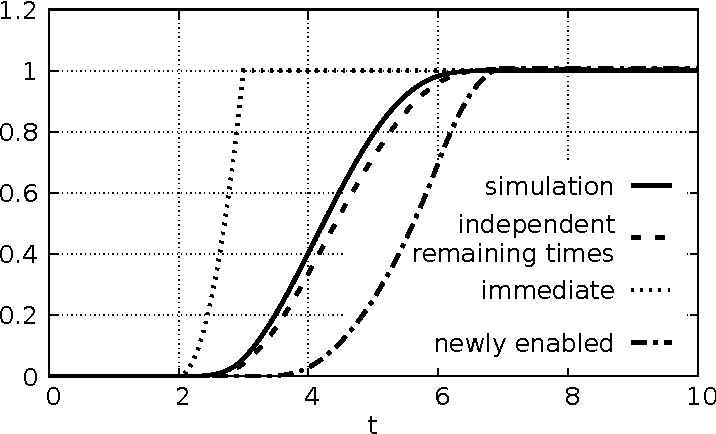
\includegraphics[scale=0.6]{simple_tti_cdf}}
      \end{center}
      
      \begin{minipage}{0.45\textwidth}
        \textit{TTIdle} computed in
        \begin{itemize}
          \item 45 min for simulation
          \item 0.18 s for bounds
        \end{itemize}
      \end{minipage}
      \begin{minipage}{0.5\textwidth}
        Due to steady-state probabilities
        \begin{itemize}
          \item steady-state probability of $0.208$
          \item $79.2\%$ of runs are discarded
        \end{itemize}
      \end{minipage}
    \end{frame}
    
    \begin{frame}{Simple assembly line}{TTDone, TTIdle, TTStartNext}
      \begin{minipage}{0.3\textwidth}
        \begin{center}
          {\tiny $F_{TTD(1,\omega)}$}\\
          \colorbox{white}{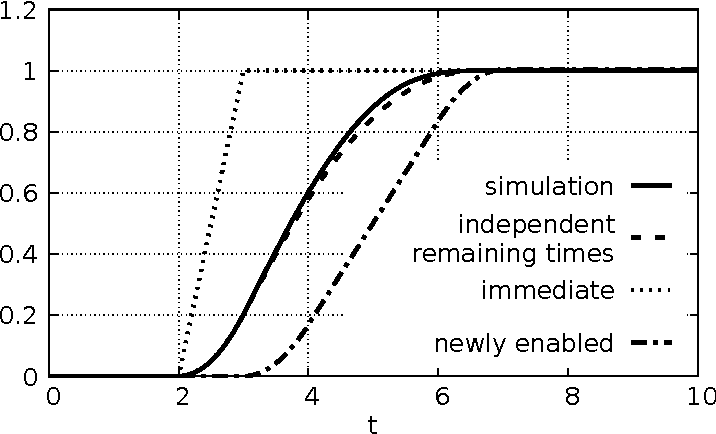
\includegraphics[scale=0.25]{simple_ttd_cdf}}
        \end{center}
      \end{minipage}
      \begin{minipage}{0.3\textwidth}
        \begin{center}
          {\tiny $F_{TTI(1,\omega)}$}\\
          \colorbox{white}{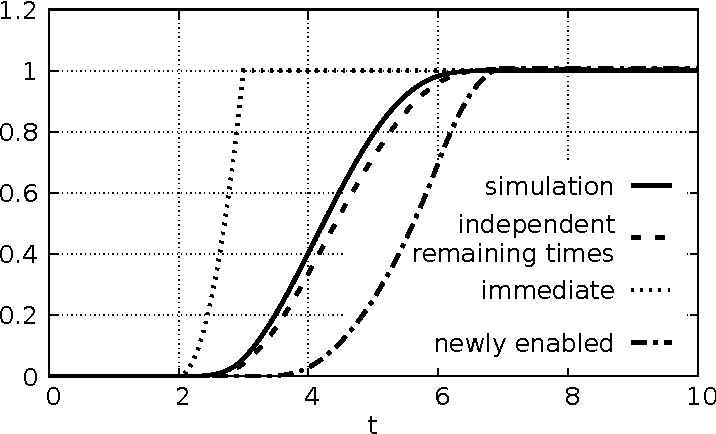
\includegraphics[scale=0.25]{simple_tti_cdf}}
        \end{center}
      \end{minipage}
      \begin{minipage}{0.3\textwidth}
        \begin{center}
          {\tiny $F_{TTSN(2,\omega)}$}\\
          \colorbox{white}{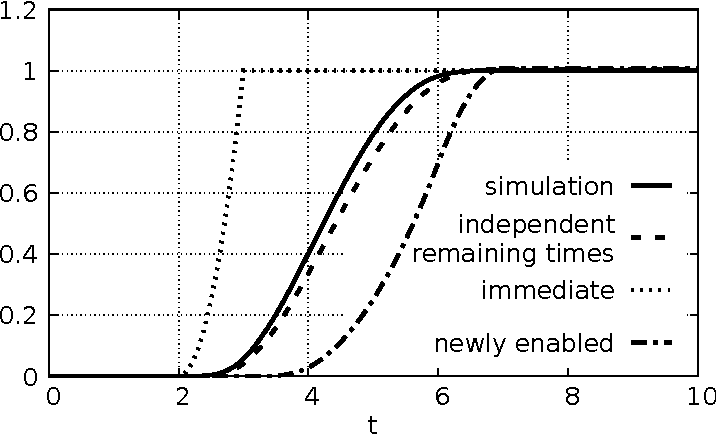
\includegraphics[scale=0.25]{simple_ttsn_cdf}}
        \end{center}
      \end{minipage}
      
      \begin{minipage}{0.5\textwidth}
        \textit{TTD}, \textit{TTI} and \textit{TTSN} computed in
        \begin{itemize}
          \item 41/45/42 min for simulation
          \item 0.15/0.18/0.10 s for bounds
        \end{itemize}
      \end{minipage}
      \begin{minipage}{0.45\textwidth}
        \vspace{2em}
        Very good approximation results
        \begin{itemize}
          \item especially for \textit{independent remaining times}
        \end{itemize}
        Feasible approach
        \begin{itemize}
          \item very fast bounds evaluation
          \item compared to simulation
        \end{itemize}
      \end{minipage}
    \end{frame}
  
  \subsection{Complex assembly line}
    \begin{frame}{Complex assembly line}{TTIdle}
        \begin{center}
          $F_{TTI(5,\omega)}$\\
          \colorbox{white}{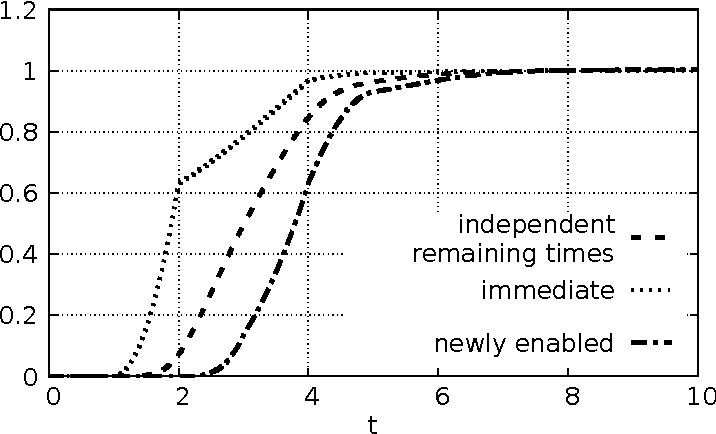
\includegraphics[scale=0.6]{complex_tti_cdf}}
        \end{center}
        
        \textit{TTIdle} computed in
        \begin{itemize}
          \item 0.123 s for bounds
        \end{itemize}
        Simulation would be too computationally expensive
    \end{frame}
  
    \begin{frame}{Complex assembly line}{TTDone, TTIdle, TTStartNext}
      \begin{minipage}{0.3\textwidth}
        \begin{center}
          {\tiny $F_{TTD(5,\omega)}$}\\
          \colorbox{white}{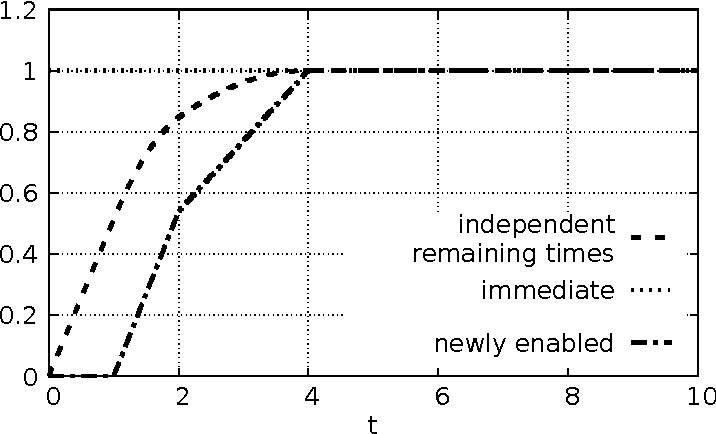
\includegraphics[scale=0.25]{complex_ttd_cdf}}
        \end{center}
      \end{minipage}
      \begin{minipage}{0.3\textwidth}
        \begin{center}
          {\tiny $F_{TTI(5,\omega)}$}\\
          \colorbox{white}{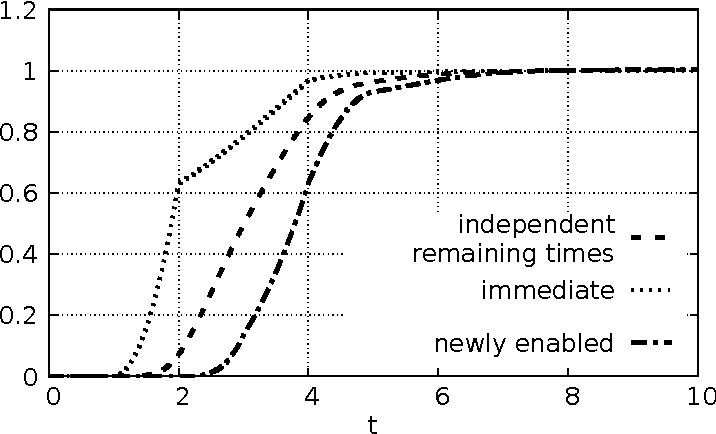
\includegraphics[scale=0.25]{complex_tti_cdf}}
        \end{center}
      \end{minipage}
      \begin{minipage}{0.3\textwidth}
        \begin{center}
          {\tiny $F_{TTSN(5,\omega)}$}\\
          \colorbox{white}{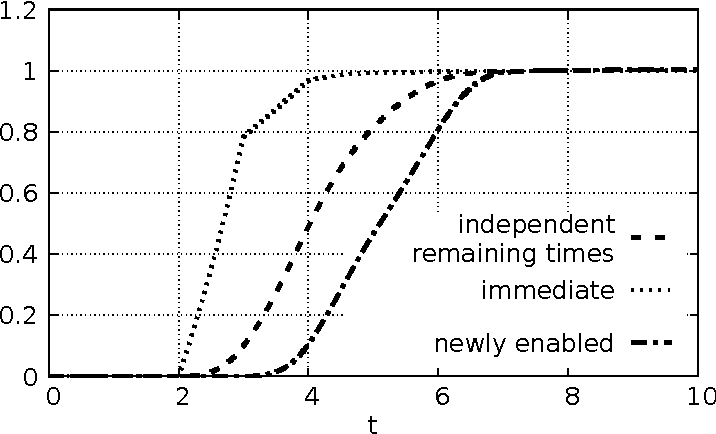
\includegraphics[scale=0.25]{complex_ttsn_cdf}}
        \end{center}
      \end{minipage}
      
      \vspace{4em}
      \begin{minipage}{0.5\textwidth}
        \textit{TTD}, \textit{TTI} and \textit{TTSN} computed in
        \begin{itemize}
          \item 0.126/0.123/0.75 s for bounds
        \end{itemize}
      \end{minipage}
      \begin{minipage}{0.45\textwidth}
        Scalable solution
        \begin{itemize}
          \item in a complex scenario
          \item simulation would be infeasible
        \end{itemize}
      \end{minipage}
    \end{frame}